\documentclass[a0,portrait]{a0poster}
%\usepackage{alltt}
\usepackage{color}
\usepackage{times}
\usepackage{a0poster}
\usepackage{graphicx}
\usepackage{epstopdf}
\usepackage{amssymb,amsmath}
\usepackage{array}
\usepackage{multirow}
\usepackage{tabularx,tabulary}

\newcommand{\ket}[1]{\left| #1\right\rangle}


%%%%%%%%%%%%%%%%%%%%%%%%%%%%%%%%%%%%%%%%%%%%%%%%%%%%%%%%%%%%%%%%%%%%%%%%%%%%%


\begin{document}

\title{Fairness in Lazy Quantum Random Walks}
\author{David F. Dolphin$^{\dagger}$ and Michael McGettrick$^*$}
\address{Department of Information Technology, National University of Ireland, Galway}
\email{\{d.dolphin1,micheal.mcgettrick\}@nuigalway.ie}

\makeheader


%% Column 1
\begin{center}
\col{
\paragraph{Introduction}
Random walks are a statistical tool, used to study patterns in randomness. They can be applied over a finite space (typically a graph) or an infinite continuum.

Quantum (random) walks are the quantum equivalent of classical random walks. They are studied to observe the statistical properties of quantum systems. These results aid in the general design of randomised quantum algorithms, particularly regarding efficiency concerns for those algorithms\cite{Ke:2003}.

Much of the work concerning discrete quantum walks deals with two-state bits, known as qubits. At each time step in a qubit system the particle must move. Our work looks at three-state systems, whose particles are known as qutrits. In a qutrit system the particle is not forced to move at each time step; there is a possibility that it can remain in the same location. This possibility to remain in place gives rise to the name ``lazy'' quantum walks.

This poster describes work in progress on this topic.

\paragraph{Classical Walks}
The most approachable application of a discrete classical random walk is a fair coin toss, the result of which moves a particle left or right on an infinite line. After this experiment has been run a number of times, the distance from the origin is recorded. This series of experiments is then run a number of times, and the distance from the origin is recorded each time. When a histogram of these results is plotted, we see that the distribution of distances from the origin is approximately normal (Figure~\ref{clas_10k}). As the particle can only land on an odd numbered space after an odd number of steps and an even numbered space after an even number of steps, over a larger number of steps every second value will be zero.

\begin{figure}
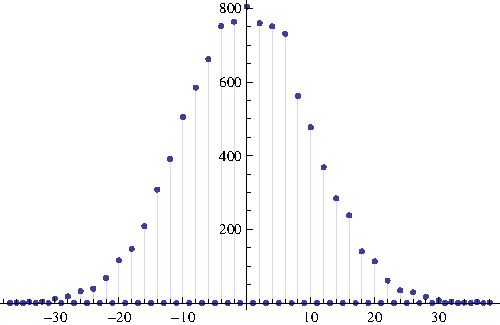
\includegraphics[height=100mm]{classic-10k-of-100-itterations.pdf}
\caption{Histogram of final positions, 10,000 iterations of 100-step classical walk.}
\label{clas_10k}
\end{figure}    

This can be generalised to show the probability of the particle being at a certain position after a certain number of steps\cite{Ke:2003}.

\begin{center}
\small
\begin{tabular}{|c||c|c|c|c|c|c|c|c|c|c|c|}
\hline 
& -5 & -4 & -3 & -2 & -1 & 0 & 1 & 2 & 3 & 4 & 5 \\
\hline \hline
\hspace*{\fill} 0 \hspace*{\fill} &  &  &  &  &  & 1 &  &  &  &  & \\
\hline 
1 &  &  &  &  & $\dfrac{ 1 }{ 2 }$ &  & $\dfrac{ 1 }{ 2 }$ &  &  &  & \hspace*{\fill} \\
\hline 
2 &  &  &  & $\dfrac{1}{4}$ &  & $\dfrac{1}{2}$ &  & $\dfrac{1}{4}$ &  &  & \hspace*{\fill} \\
\hline 
3 &  &  &  $\dfrac{1}{8}$ &  & $\dfrac{3}{8}$ &  & $\dfrac{3}{8}$ &  & $\dfrac{1}{8}$  &  & \hspace*{\fill} \\
\hline 
4 &  & \hspace*{\fill} $\dfrac{1}{16}$ \hspace*{\fill} &  & \hspace*{\fill} $\dfrac{1}{4}$ \hspace*{\fill} &  & \hspace*{\fill} $\dfrac{3}{8}$ \hspace*{\fill} &  & \hspace*{\fill} $\dfrac{1}{4}$ \hspace*{\fill} &  & \hspace*{\fill} $\dfrac{1}{16}$ \hspace*{\fill} & \hspace*{\fill} \\
\hline 
5 & \hspace*{\fill} $\dfrac{1}{32}$ \hspace*{\fill} &  & \hspace*{\fill} $\dfrac{5}{32}$ \hspace*{\fill} &  & \hspace*{\fill} $\dfrac{5}{16}$ \hspace*{\fill} &  & \hspace*{\fill} $\dfrac{5}{16}$ \hspace*{\fill} &  & \hspace*{\fill} $\dfrac{5}{32}$ \hspace*{\fill} &  & \hspace*{\fill} $\dfrac{1}{32}$ \hspace*{\fill} \\
\hline 
\end{tabular}
\end{center}

\begin{figure}
\caption{The probability of being at node $i$ after $T$ steps of the classical random walk on the line starting in 0.}
\label{clas_ti}
\end{figure}    

However, on a closed graph the probabilities converge over time. On a cyclic graph with 4 nodes, where we can move clockwise or counter-clockwise after each time-step, the probabilities converge to $\frac{1}{4}$ for each of the four nodes.

We now consider a three state system on the integers. A particle can move left, right or remain stationary at each time step. Figure~\ref{clas2_ti} shows the generalised probability distributions of a lazy classical walk.

\begin{center}
\small
\begin{tabular}{|c||c|c|c|c|c|c|c|c|c|c|c|}
\hline 
& -5 & -4 & -3 & -2 & -1 & 0 & 1 & 2 & 3 & 4 & 5 \\
\hline \hline
\hspace*{\fill} 0 \hspace*{\fill} &  &  &  &  &  & 1 &  &  &  &  & \\
\hline 
1 &  &  &  &  & 
$\dfrac{ 1 }{ 3 }$ &
$\dfrac{ 1 }{ 3 }$ &
$\dfrac{ 1 }{ 3 }$ &  &  &  & 
\hspace*{\fill} \\
\hline 
2 &  &  &  & 
$\dfrac{1}{9}$ & 
$\dfrac{ 2 }{ 9 }$ & 
$\dfrac{1}{3}$ & 
$\dfrac{ 2 }{ 9 }$ & 
$\dfrac{1}{9}$ &  &  & 
\hspace*{\fill} \\
\hline 
3 &  &  &  
$\dfrac{1}{27}$ &  
$\dfrac{ 1 }{ 9 }$ & 
$\dfrac{2}{9}$ &  
$\dfrac{ 2 }{ 27 }$ & 
$\dfrac{2}{9}$ &  
$\dfrac{ 1 }{ 9 }$ & 
$\dfrac{1}{27}$  &  & 
\hspace*{\fill} \\
\hline 
4 &  &
\hspace*{\fill} $\dfrac{1}{81}$ \hspace*{\fill} & 
$\dfrac{ 4 }{ 81 }$ & 
\hspace*{\fill} $\dfrac{10}{81}$ \hspace*{\fill} &  
$\dfrac{ 16 }{ 81 }$ & 
\hspace*{\fill} $\dfrac{19}{81}$ \hspace*{\fill} &  
$\dfrac{ 16 }{ 81 }$ & 
\hspace*{\fill} $\dfrac{10}{81}$ \hspace*{\fill} &  
$\dfrac{ 4 }{ 81 }$ & 
\hspace*{\fill} $\dfrac{1}{81}$ \hspace*{\fill} & 
\hspace*{\fill} \\
\hline 
5 & 
\hspace*{\fill} $\dfrac{1}{243}$ \hspace*{\fill} & 
$\dfrac{ 5 }{ 243 }$ & 
\hspace*{\fill} $\dfrac{5}{81}$ \hspace*{\fill} & 
$\dfrac{ 10 }{ 81 }$ & 
\hspace*{\fill} $\dfrac{5}{27}$ \hspace*{\fill} & 
$\dfrac{ 17 }{ 81 }$ & 
\hspace*{\fill} $\dfrac{5}{27}$ \hspace*{\fill} & 
$\dfrac{ 10 }{ 81 }$ & 
\hspace*{\fill} $\dfrac{5}{81}$ \hspace*{\fill} & 
$\dfrac{ 5 }{ 243 }$ & 
\hspace*{\fill} $\dfrac{1}{243}$ \hspace*{\fill} \\
\hline 
\end{tabular}
\end{center}

\begin{figure}
\caption{The probability of being at position $i$ after $T$ steps of the lazy classical random walk on the line starting in 0.}
\label{clas2_ti}
\end{figure}    

}
%% Column 2
\col{ 
\paragraph{}
The lazy classical walk has a normal distribution; the introduction of the lazy step removes the odd/even restriction. Like the standard classical walk, the lazy classical walk converges to equal values on a closed graph.

It is possible to vary the lazy bias of a classical walk. A common bias is to choose a probability per iteration of $\frac{1}{2}$ for the lazy move, $\frac{1}{4}$ for the clockwise move, and $\frac{1}{4}$ for the counter-clockwise move. This bias can be modelled as two coin tosses, where one coin signals movement or its absence, the second signals the direction of movement (if the first coin signals movement).

However, we have chosen to give each movement possibility a probability of $\frac{1}{3}$. This is for comparison with the quantum randomization function we will be examining.

\paragraph{Hadamard Gate}

The quantum randomizing function we are examining is known as a Hadamard Gate (also known as a Hadamard Coin). A coin used for a two-state (qubit) system is $H_2$ 

\begin{equation}
H_2 = \dfrac{1}{\sqrt{2}} \begin{pmatrix}
  1 & 1 \\
  1 & -1 
\end{pmatrix}
\label{eq:1}
\end{equation}

It is unitary and has been shown\cite{Ke:2003} to be fair. 

The Hadamard gate has been generalised by Marttala\cite{Ma:2007} to $H_m$, where $m$ is the number of states in the system. 

As we are interested in a lazy walk we want a three-state gate $H_3$, where the three states represent a left movement, a right movement, and no movement.

\begin{equation}
H_3 = \dfrac{1}{\sqrt{3}} \begin{pmatrix}
  1 & 1 & 1 \\
  1 & -(-1)^{\frac{1}{3}} & (-1)^{\frac{2}{3}} \\
  1 & (-1)^{\frac{2}{3}} & -(-1)^{\frac{1}{3}}
\end{pmatrix}
\label{eq:5}
\end{equation}

We are satisfied that $H_3$ is unitary as 

\begin{equation}
H_{3}H_{3}^{\dagger} = I_3
\label{eq:6}
\end{equation}

\paragraph{Quantum Walks on a Graph}

A Lazy One-Dimensional Discrete Quantum Walk takes place on the state space spanned by vectors
\begin{equation}
\ket{n,p}
\label{eq:7}
\end{equation}
where $n\in Z$
and $p\in \{0,1,2\}$ is a three-state variable. $n$ represents the position of a particle on the walk and is the walk's classical component. $p$ is the quantum component; it is typically a two-state spin, but we have added a third state to represent our lazy state. 

One step of the walk is given by the transitions
\begin{eqnarray}
\ket{n,0} &\longrightarrow a\ket{n,0} + b\ket{n+1,1} + c\ket{n-1,2}\\
\ket{n,1} &\longrightarrow d\ket{n,0} + e\ket{n+1,1} + f\ket{n-1,2}\\
\ket{n,2} &\longrightarrow g\ket{n,0} + h\ket{n+1,1} + i\ket{n-1,2}
\end{eqnarray} 
where 
\begin{equation}
\begin{pmatrix}
  a & b & c \\
  d & e & f \\
  g & h & i 
\end{pmatrix} = H_3
\end{equation}

This has been expanded from the two-state walk equations given elsewhere\cite{Ke:2003,Mc:2010}.

\begin{figure}
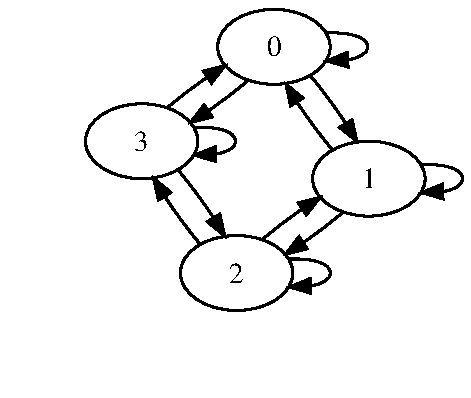
\includegraphics[height=140mm]{std-1.pdf}
\caption{State transition diagram for cycle of length four.}
\label{std_10k}
\end{figure}    

Multiple randomising iterations were performed for a cyclic graph with four nodes and no directional biasing. Different initial states were used to obtain a variety of results. A non-lazy walk on a cycle with four nodes was also analysed for comparison to the lazy results.
}
%% Column 3
\col{
\paragraph{Results}
The non-lazy cycle converges to $\frac{1}{4}$ for each vertex. This is due to the fact that the nodal probabilities repeat after 8 steps, caused by constructive and destructive interference on the graph.

\begin{center}
\small
\begin{tabular}{|c||c|c|c|c|c|c|c|c|c|c|c|}
\hline 
& $\ket{0,0}$ & $\ket{0,1}$ & $\ket{1,0}$ & $\ket{1,1}$ & $\ket{2,0}$ & $\ket{2,1}$ & $\ket{3,0}$ & $\ket{3,1}$ \\
\hline \hline
\hspace*{\fill} 0 \hspace*{\fill} & 1  &  &  &  &  &  & & \\
\hline 
1 &  &  &  &  
$\dfrac{ 1 }{ \sqrt{2} }$ & & &
$\dfrac{ 1 }{ \sqrt{2} }$  & 
\hspace*{\fill} \\
\hline 
2 &  
$\dfrac{ 1 }{ 2 }$ & 
$\dfrac{ 1 }{ 2 }$ & & &
$\dfrac{ 1 }{ 2 }$ & 
$-\dfrac{ 1 }{ 2 }$ & & &
\hspace*{\fill} \\
\hline 
3 & & & & & & & 
$\dfrac{ 1 }{ \sqrt{2} }$ & 
$\dfrac{ 1 }{ \sqrt{2} }$
\hspace*{\fill} \\
\hline
\hspace*{\fill} 4 \hspace*{\fill} &  &  &  &  & 1 &  & & \\
\hline 
\end{tabular}
\end{center}

\begin{figure}
\caption{The probability of being at position $i$ after $T$ steps of the quantum random walk on a cycle with four nodes, starting at $\ket{0,0}$.}
\label{quan_ti}
\end{figure}    

As a result, the nodal probabilities converge to equal values for all nodes on a four node cycle for a classical walk, lazy and non-lazy, and a non-lazy quantum walk. However, the nodal probabilities do not converge to equal values for the lazy quantum walk on a cyclic graph with four nodes.

We define our initial state as 

\begin{equation}
x\ket{0,0}+y\ket{0,1}+y\ket{0,2}
\end{equation}

\begin{equation}
y=\sqrt{\frac{1-x^2}{2}}
\end{equation}

\begin{figure}
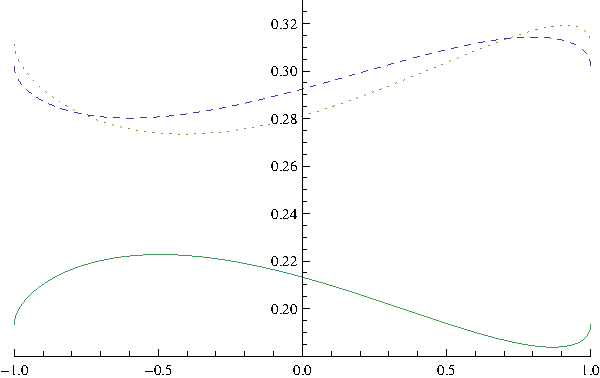
\includegraphics[height=45mm]{xyy-100-steps-1-1.pdf}
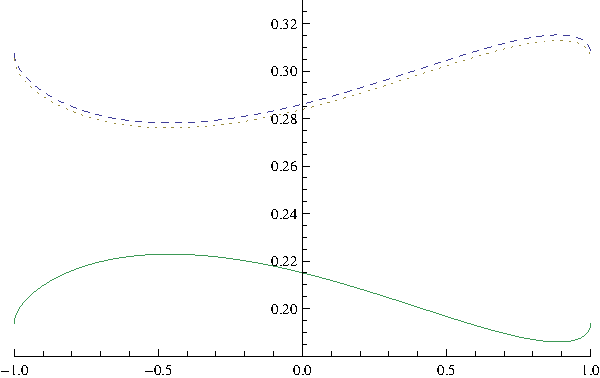
\includegraphics[height=45mm]{xyy-500-steps-1-1.pdf}
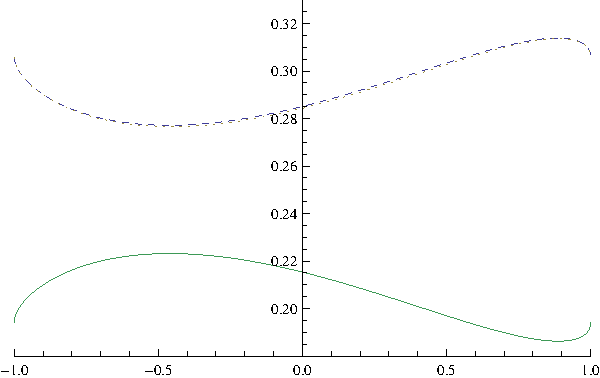
\includegraphics[height=140mm]{xyy-2000-steps-1-1.pdf}
  \caption{Final value of nodal probability for each node in a 4 node cycle after a number of iterations of the lazy quantum walk, with x varying from $-1$ to $1$. Values are for Node 0 (dashed), 1 \& 3 (solid), and 2 (dotted). Results are for 100(top left), 500(top right), and 2000(bottom) iterations.}
\label{trends}
\end{figure}

\begin{center}
\small
\begin{tabular}{|c||c|c|c|c|}
\hline 
\multirow{2}{*}{ }& \multicolumn{2}{ |c| }{\hspace*{\fill} Minimum Probability \hspace*{\fill} }  &
 \multicolumn{2}{ |c| }{\hspace*{\fill} Maximum Probability \hspace*{\fill} } \\
\hline 
& \hspace*{\fill} x-value \hspace*{\fill} 
& \hspace*{\fill} Probability \hspace*{\fill} 
& \hspace*{\fill} x-value \hspace*{\fill} 
& \hspace*{\fill} Probability\hspace*{\fill} \\
\hline \hline
\hspace*{\fill} Node 0 \hspace*{\fill} 
& \hspace*{\fill} -0.464476 \hspace*{\fill} 
& \hspace*{\fill} 0.277144 \hspace*{\fill} 
& \hspace*{\fill} 0.885579 \hspace*{\fill} 
& \hspace*{\fill} 0.313895 \hspace*{\fill} \\
\hline
\hspace*{\fill} Node's 1\& 3 \hspace*{\fill} &
0.887671 & 0.186246 &
\hspace*{\fill} -0.460463 \hspace*{\fill}& 
0.223129\\
\hline 
Node 2 & -0.45647 & 0.276597 & 0.889731 & 0.313614\\
\hline 
\end{tabular}
\end{center}

\begin{figure}
\caption{The maximum and minimum positional probabilities for each position after 2000 iterations.}
\label{quan_max}
\end{figure}    

\paragraph{Conclusion and extensions}

The Hadamard gate is commonly considered to be fair and balanced. It produces some results equal to those obtained from a fair classical coin, and some different.

We have investigated initial states with real coefficients, but intend on also looking at the results when complex coefficients are used.

We have only investigated a cycle with four nodes. The profile of $x$ vs. probability values may be unique to a lazy quantum walks on a cycle with four nodes, an odd number of nodes or may be common to all graphs. We intend on investigating cycles with more vertices.

The values for Position 0 and 2 look likely to converge. We intend to investigate if these positional profiles do converge. We also intend to find the maximum and minimum cumulative probabilities for each vertex.

\references
\bibliography{jm.ref}
}
\end{center}


\makefooter

\end{document}

